% !TeX spellcheck = pl_PL
%%%%%%%%%%%%%%%%%%%%%%%%%%%%%%%%%%%%%%%%%%%
%                                        %
% Szablon pracy dyplomowej magisterskiej %
% zgodny  z aktualnymi  przepisami  SZJK %
%                                        %
%%%%%%%%%%%%%%%%%%%%%%%%%%%%%%%%%%%%%%%%%%
%                                        %
%  (c) Krzysztof Simiński, 2018-2023     %
%                                        %
%%%%%%%%%%%%%%%%%%%%%%%%%%%%%%%%%%%%%%%%%%
%                                        %
% Najnowsza wersja szablonów jest        %
% podstępna pod adresem                  %
% github.com/ksiminski/polsl-aei-theses  %
%                                        %
%%%%%%%%%%%%%%%%%%%%%%%%%%%%%%%%%%%%%%%%%%
%
%
% Projekt LaTeXowy zapewnia odpowiednie formatowanie pracy,
% zgodnie z wymaganiami Systemu zapewniania jakości kształcenia.
% Proszę nie zmieniać ustawień formatowania (np. fontu,
% marginesów, wytłuszczeń, kursywy itd. ).
%
% Projekt można kompilować na kilka sposobów.
%
% 1. kompilacja pdfLaTeX
%
% pdflatex main
% bibtex   main
% pdflatex main
% pdflatex main
%
%
% 2. kompilacja XeLaTeX
%
% Kompilatacja przy użyciu XeLaTeXa różni się tym, że na stronie
% tytułowej używany jest font Calibri. Wymaga to jego uprzedniego
% zainstalowania.
%
% xelatex main
% bibtex  main
% xelatex main
% xelatex main
%
%
%%%%%%%%%%%%%%%%%%%%%%%%%%%%%%%%%%%%%%%%%%%%%%%%%%%%%
% W przypadku pytań, uwag, proszę pisać na adres:   %
%      krzysztof.siminski(małpa)polsl.pl            %
%%%%%%%%%%%%%%%%%%%%%%%%%%%%%%%%%%%%%%%%%%%%%%%%%%%%%
%
% Chcemy ulepszać szablony LaTeXowe prac dyplomowych.
% Wypełniając ankietę spod poniższego adresu pomogą
% Państwo nam to zrobić. Ankieta jest całkowicie
% anonimowa. Dziękujemy!


% https://docs.google.com/forms/d/e/1FAIpQLScyllVxNKzKFHfILDfdbwC-jvT8YL0RSTFs-s27UGw9CKn-fQ/viewform?usp=sf_link
%
%%%%%%%%%%%%%%%%%%%%%%%%%%%%%%%%%%%%%%%%%%%%%%%%%%%%%%%%%%%%%%%%%%%%%%%%%

%%%%%%%%%%%%%%%%%%%%%%%%%%%%%%%%%%%%%%%%%%%%%%%
%                                             %
% PERSONALIZACJA PRACY - DANE PRACY           %
%                                             %
%%%%%%%%%%%%%%%%%%%%%%%%%%%%%%%%%%%%%%%%%%%%%%%

% Proszę wpisać swoje dane w poniższych definicjach.

% TODO
% dane autora
\newcommand{\FirstNameAuthor}{Jakub}
\newcommand{\SurnameAuthor}{Kula}
\newcommand{\IdAuthor}{296849}   % numer albumu  (bez $\langle$ i $\rangle$)

% drugi autor:
%\newcommand{\FirstNameCoauthor}{Imię}   % Jeżeli jest drugi autor, to tutaj należy podać imię.
%\newcommand{\SurnameCoauthor}{Nazwisko} % Jeżeli jest drugi autor, to tutaj należy podać nazwisko.
%\newcommand{\IdCoauthor}{$\langle$wpisać właściwy$\rangle$}  % numer albumu drugiego autora (bez $\langle$ i $\rangle$)
% Gdy nie ma drugiego autora, należy zostawić poniższe definicje puste, jak poniżej. Gdy jest drugi autor, należy zakomentować te linie.
\newcommand{\FirstNameCoauthor}{} % Jeżeli praca ma tylko jednego autora, to dane drugiego autora zostają puste.
\newcommand{\SurnameCoauthor}{}   % Jeżeli praca ma tylko jednego autora, to dane drugiego autora zostają puste.
\newcommand{\IdCoauthor}{}  % Jeżeli praca ma tylko jednego autora, to dane drugiego autora zostają puste.
%%%%%%%%%%

\newcommand{\Supervisor}{dr hab. inż. Pander Tomasz, prof. PŚ}     % dane promotora (bez $\langle$ i $\rangle$)
\newcommand{\Title}{Zastosowanie metod sztucznej inteligencji do detekcji arytmii na podstawie sygnałów PPG}           % tytuł pracy po polsku
\newcommand{\TitleAlt}{Application of artificial intelligence methods for arrhythmia detection based on PPG signal}                     % thesis title in English
\newcommand{\Program}{Informatyka}            % kierunek studiów  (bez $\langle$ i $\rangle$)
\newcommand{\Specialisation}{Internet i technologie sieciowe}     % specjalność  (bez $\langle$ i $\rangle$)
\newcommand{\Departament}{Cybernetyki, Nanotechnologii i Przetwarzania Danych}        % katedra promotora  (bez $\langle$ i $\rangle$)

% Jeżeli został wyznaczony promotor pomocniczy lub opiekun, proszę go/ją wpisać ...
\newcommand{\Consultant}{} % dane promotora pomocniczego, opiekuna (bez $\langle$ i $\rangle$)
% ... w przeciwnym razie proszę zostawić puste miejsce jak poniżej:
%\newcommand{\Consultant}{} % brak promotowa pomocniczego / opiekuna

% koniec fragmentu do modyfikacji
%%%%%%%%%%%%%%%%%%%%%%%%%%%%%%%%%%%%%%%%%%


%%%%%%%%%%%%%%%%%%%%%%%%%%%%%%%%%%%%%%%%%%%%%%%
%                                             %
% KONIEC PERSONALIZACJI PRACY                 %
%                                             %
%%%%%%%%%%%%%%%%%%%%%%%%%%%%%%%%%%%%%%%%%%%%%%%

%%%%%%%%%%%%%%%%%%%%%%%%%%%%%%%%%%%%%%%%


%%%%%%%%%%%%%%%%%%%%%%%%%%%%%%%%%%%%%%%%%%%%%%%
%                                             %
% PROSZĘ NIE MODYFIKOWAĆ PONIŻSZYCH USTAWIEŃ! %
%                                             %
%%%%%%%%%%%%%%%%%%%%%%%%%%%%%%%%%%%%%%%%%%%%%%%



\documentclass[a4paper,twoside,12pt]{book}
\usepackage[utf8]{inputenc}
\usepackage[T1]{fontenc}
\usepackage{amsmath,amsfonts,amssymb,amsthm}
\usepackage[british,polish]{babel}
\usepackage{indentfirst}
\usepackage{xurl}
\usepackage{xstring}
\usepackage{ifthen}

\usepackage{makecell}
\usepackage{siunitx}
\usepackage{tikz}


\usepackage{ifxetex}

\ifxetex
	\usepackage{fontspec}
	\defaultfontfeatures{Mapping=tex—text} % to support TeX conventions like ``——-''
	\usepackage{xunicode} % Unicode support for LaTeX character names (accents, European chars, etc)
	\usepackage{xltxtra} % Extra customizations for XeLaTeX
\else
	\usepackage{lmodern}
\fi



\usepackage[margin=2.5cm]{geometry}
\usepackage{graphicx}
\usepackage{hyperref}
\usepackage{booktabs}
\usepackage{tikz}
\usepackage{pgfplots}
\usepackage{mathtools}
\usepackage{geometry}
\usepackage{subcaption}   % subfigures
\usepackage[page]{appendix} % toc,
\renewcommand{\appendixtocname}{Dodatki}
\renewcommand{\appendixpagename}{Dodatki}
\renewcommand{\appendixname}{Dodatek}

\usepackage{csquotes}
\usepackage[natbib=true,backend=bibtex,maxbibnames=99]{biblatex}  % kompilacja bibliografii BibTeXem
%\usepackage[natbib=true,backend=biber,maxbibnames=99]{biblatex}  % kompilacja bibliografii Biberem
\bibliography{biblio}

\usepackage{ifmtarg}   % empty commands  

\usepackage{setspace}
\onehalfspacing


\frenchspacing



%%%% TODO LIST GENERATOR %%%%%%%%%

\usepackage{color}
\definecolor{brickred}      {cmyk}{0   , 0.89, 0.94, 0.28}

\makeatletter \newcommand \kslistofremarks{\section*{Uwagi} \@starttoc{rks}}
\newcommand\l@uwagas[2]
{\par\noindent \textbf{#2:} %\parbox{10cm}
	{#1}\par} \makeatother



\newcommand{\ksremark}[1]{%
	{%\marginpar{\textdbend}
			{\color{brickred}{[#1]}}}%
	\addcontentsline{rks}{uwagas}{\protect{#1}}%
}

\newcommand{\comma}{\ksremark{przecinek}}
\newcommand{\nocomma}{\ksremark{bez przecinka}}
\newcommand{\styl}{\ksremark{styl}}
\newcommand{\ortografia}{\ksremark{ortografia}}
\newcommand{\fleksja}{\ksremark{fleksja}}
\newcommand{\pauza}{\ksremark{pauza `--', nie dywiz `-'}}
\newcommand{\kolokwializm}{\ksremark{kolokwializm}}
\newcommand{\cudzyslowy}{\ksremark{,,polskie cudzysłowy''}}

%%%%%%%%%%%%%% END OF TODO LIST GENERATOR %%%%%%%%%%%

\newcommand{\printCoauthor}{%		
	\StrLen{\FirstNameCoauthor}[\FNCoALen]
	\ifthenelse{\FNCoALen > 0}%
	{%
		{\large\bfseries\Coauthor\par}

			{\normalsize\bfseries \LeftId: \IdCoauthor\par}
	}%
	{}
}

%%%%%%%%%%%%%%%%%%%%%
\newcommand{\autor}{%		
	\StrLen{\FirstNameCoauthor}[\FNCoALenXX]
	\ifthenelse{\FNCoALenXX > 0}%
	{\FirstNameAuthor\ \SurnameAuthor, \FirstNameCoauthor\ \SurnameCoauthor}%
	{\FirstNameAuthor\ \SurnameAuthor}%
}
%%%%%%%%%%%%%%%%%%%%%

\StrLen{\FirstNameCoauthor}[\FNCoALen]
\ifthenelse{\FNCoALen > 0}%
{%
	\author{\FirstNameAuthor\ \SurnameAuthor, \FirstNameCoauthor\ \SurnameCoauthor}
}%
{%
	\author{\FirstNameAuthor\ \SurnameAuthor}
}%

%%%%%%%%%%%% ZYWA PAGINA %%%%%%%%%%%%%%%
% brak kapitalizacji zywej paginy
\usepackage{fancyhdr}
\pagestyle{fancy}
\fancyhf{}
\fancyhead[LO]{\nouppercase{\it\rightmark}}
\fancyhead[RE]{\nouppercase{\it\leftmark}}
\fancyhead[LE,RO]{\it\thepage}


\fancypagestyle{tylkoNumeryStron}{%
	\fancyhf{}
	\fancyhead[LE,RO]{\it\thepage}
}

\fancypagestyle{bezNumeracji}{%
	\fancyhf{}
	\fancyhead[LE,RO]{}
}


\fancypagestyle{NumeryStronNazwyRozdzialow}{%
	\fancyhf{}
	\fancyhead[LE]{\nouppercase{\autor}}
	\fancyhead[RO]{\nouppercase{\leftmark}}
	\fancyfoot[CE, CO]{\thepage}
}


%%%%%%%%%%%%% OBCE WTRETY  
\newcommand{\obcy}[1]{\emph{#1}}
\newcommand{\english}[1]{{\selectlanguage{british}\obcy{#1}}}
%%%%%%%%%%%%%%%%%%%%%%%%%%%%%

% polskie oznaczenia funkcji matematycznych
\renewcommand{\tan}{\operatorname {tg}}
\renewcommand{\log}{\operatorname {lg}}

% jeszcze jakies drobiazgi

\newcounter{stronyPozaNumeracja}

%%%%%%%%%%%%%%%%%%%%%%%%%%% 
\newcommand{\printOpiekun}[1]{%		

	\StrLen{\Consultant}[\mystringlen]
	\ifthenelse{\mystringlen > 0}%
	{%
		{\large{\bfseries OPIEKUN, PROMOTOR POMOCNICZY}\par}

			{\large{\bfseries \Consultant}\par}
	}%
	{}
}
%
%%%%%%%%%%%%%%%%%%%%%%%%%%%%%%%%%%%%%%%%%%%%%%

% Proszę nie modyfikować poniższych definicji!
\newcommand{\Author}{\FirstNameAuthor\ \MakeUppercase{\SurnameAuthor}}
\newcommand{\Coauthor}{\FirstNameCoauthor\ \MakeUppercase{\SurnameCoauthor}}
\newcommand{\Type}{PRACA MAGISTERSKA}
\newcommand{\Faculty}{Wydział Automatyki, Elektroniki i Informatyki}
\newcommand{\Polsl}{Politechnika Śląska}
\newcommand{\Logo}{politechnika_sl_logo_bw_pion_pl.pdf}
\newcommand{\LeftId}{Nr albumu}
\newcommand{\LeftProgram}{Kierunek}
\newcommand{\LeftSpecialisation}{Specjalność}
\newcommand{\LeftSUPERVISOR}{PROWADZĄCY PRACĘ}
\newcommand{\LeftDEPARTMENT}{KATEDRA}
%%%%%%%%%%%%%%%%%%%%%%%%%%%%%%%%%%%%%%%%%%%%%%

%%%%%%%%%%%%%%%%%%%%%%%%%%%%%%%%%%%%%%%%%%%%%%%
%                                             %
% KONIEC USTAWIEŃ                             %
%                                             %
%%%%%%%%%%%%%%%%%%%%%%%%%%%%%%%%%%%%%%%%%%%%%%%




%%%%%%%%%%%%%%%%%%%%%%%%%%%%%%%%%%%%%%%%%%%%%%%
%                                             %
% MOJE PAKIETY, USTAWIENIA ITD                %
%                                             %
%%%%%%%%%%%%%%%%%%%%%%%%%%%%%%%%%%%%%%%%%%%%%%%

% Tutaj proszę umieszczać swoje pakiety, makra, ustawienia itd.



%%%%%%%%%%%%%%%%%%%%%%%%%%%%%%%%%%%%%%%%%%%%%%%%%%%%%%%%%%%%%%%%%%%%%
% listingi i fragmentu kodu źródłowego 
% pakiet: listings lub minted
% % % % % % % % % % % % % % % % % % % % % % % % % % % % % % % % % % % 

% biblioteka listings
\usepackage{listings}
\lstset{%
	morekeywords={string,exception,std,vector},% słowa kluczowe rozpoznawane przez pakiet listings
	language=C++,% C, Matlab, Python, SQL, TeX, XML, bash, ... - vide https://www.ctan.org/pkg/listings
	commentstyle=\textit,%
	identifierstyle=\textsf,%
	keywordstyle=\sffamily\bfseries, %\texttt, %
	%captionpos=b,%
	tabsize=3,%
	frame=lines,%
	numbers=left,%
	numberstyle=\tiny,%
	numbersep=5pt,%
	breaklines=true,%
	escapeinside={@*}{*@},%
}

% % % % % % % % % % % % % % % % % % % % % % % % % % % % % % % % % % % 
% pakiet minted
%\usepackage{minted}

% pakiet wymaga specjalnego kompilowania:
% pdflatex -shell-escape main.tex
% xelatex  -shell-escape main.tex

%\usepackage[chapter]{minted} % [section]
%%\usemintedstyle{bw}   % czarno-białe kody 
%
%\setminted % https://ctan.org/pkg/minted
%{
%%fontsize=\normalsize,%\footnotesize,
%%captionpos=b,%
%tabsize=3,%
%frame=lines,%
%framesep=2mm,
%numbers=left,%
%numbersep=5pt,%
%breaklines=true,%
%escapeinside=@@,%
%}

%%%%%%%%%%%%%%%%%%%%%%%%%%%%%%%%%%%%%%%%%%%%%%%%%%%%%%%%%%%%%%%%%%%%%



%%%%%%%%%%%%%%%%%%%%%%%%%%%%%%%%%%%%%%%%%%%%%%%
%                                             %
% KONIEC MOICH USTAWIEŃ                       %
%                                             %
%%%%%%%%%%%%%%%%%%%%%%%%%%%%%%%%%%%%%%%%%%%%%%%



%%%%%%%%%%%%%%%%%%%%%%%%%%%%%%%%%%%%%%%%


\begin{document}
%\kslistofremarks

\frontmatter

%%%%%%%%%%%%%%%%%%%%%%%%%%%%%%%%%%%%%%%%%%%%%%%
%                                             %
% PROSZĘ NIE MODYFIKOWAĆ STRONY TYTUŁOWEJ!    %
%                                             %
%%%%%%%%%%%%%%%%%%%%%%%%%%%%%%%%%%%%%%%%%%%%%%%


%%%%%%%%%%%%%%%%%%  STRONA TYTUŁOWA %%%%%%%%%%%%%%%%%%%
\pagestyle{empty}
{
	\newgeometry{top=1.5cm,%
		bottom=2.5cm,%
		left=3cm,
		right=2.5cm}

	\ifxetex
		\begingroup
		\setsansfont{Calibri}

	\fi
	\sffamily
	\begin{center}
		\includegraphics[width=50mm]{\Logo}


		{\Large\bfseries\Type\par}

		\vfill  \vfill

		{\large\Title\par}

		\vfill

		{\large\bfseries\Author\par}

		{\normalsize\bfseries \LeftId: \IdAuthor}

		\printCoauthor

		\vfill

		{\large{\bfseries \LeftProgram:} \Program\par}

		{\large{\bfseries \LeftSpecialisation:} \Specialisation\par}

		\vfill  \vfill 	\vfill 	\vfill 	\vfill 	\vfill 	\vfill

		{\large{\bfseries \LeftSUPERVISOR}\par}

		{\large{\bfseries \Supervisor}\par}

		{\large{\bfseries \LeftDEPARTMENT\ \Departament} \par}

		{\large{\bfseries \Faculty}\par}

		\vfill  \vfill


		\printOpiekun{\Consultant}

		\vfill  \vfill

		{\large\bfseries  Gliwice \the\year}

	\end{center}
	\ifxetex
		\endgroup
	\fi
	\restoregeometry
}

%%%%%%%%%%%%%%%%%%%%%%%%%%%%%%%%%%%%%%%%%%%%%%%
%                                             %
% KONIEC STRONY TYTUŁOWEJ                     %
%                                             %
%%%%%%%%%%%%%%%%%%%%%%%%%%%%%%%%%%%%%%%%%%%%%%%  


\cleardoublepage

\rmfamily\normalfont
\pagestyle{empty}


%%% No to zaczynamy pisać pracę :-) %%%%

% TODO
\subsubsection*{Tytuł pracy}
\Title

\subsubsection*{Streszczenie}
(Streszczenie pracy - odpowiednie pole w systemie APD powinno zawierać kopię tego streszczenia.)

\subsubsection*{Słowa kluczowe}
(2-5 slow (fraz) kluczowych, oddzielonych przecinkami)

\subsubsection*{Thesis title}
\begin{otherlanguage}{british}
	\TitleAlt
\end{otherlanguage}

\subsubsection*{Abstract}
\begin{otherlanguage}{british}
	(Thesis abstract - to be copied into an appropriate field during an electronic submission - in English.)
\end{otherlanguage}
\subsubsection*{Key words}
\begin{otherlanguage}{british}
	(2-5 keywords, separated by commas)
\end{otherlanguage}




%%%%%%%%%%%%%%%%%% SPIS TRESCI %%%%%%%%%%%%%%%%%%%%%%
% Add \thispagestyle{empty} to the toc file (main.toc), because \pagestyle{empty} doesn't work if the TOC has multiple pages
\addtocontents{toc}{\protect\thispagestyle{empty}}
\tableofcontents

%%%%%%%%%%%%%%%%%%%%%%%%%%%%%%%%%%%%%%%%%%%%%%%%%%%%%
\setcounter{stronyPozaNumeracja}{\value{page}}
\mainmatter
\pagestyle{empty}

\cleardoublepage

\pagestyle{NumeryStronNazwyRozdzialow}

%%%%%%%%%%%%%% wlasciwa tresc pracy %%%%%%%%%%%%%%%%%

% TODO
\chapter{Wstęp}
\section{Cel i zakres pracy}
\section{Aktualny stan wiedzy}
\section{Charakterystyka rozdziałów}

% TODO

\chapter{Charakterystyka arytmii serca i sygnału PPG}
\section{Klasyfikacja i mechanizmy arytmii serca}
\subsection{Arytmie nadkomorowe}
\subsection{Arytmie komorowe}
\subsection{Migotanie przedsionków}
\section{Fotopletyzmografia - zasada działania i zastosowania}

\chapter{Metody uczenia maszynowego}
\section{Klasyczne metody}
\begin{itemize}
	\item \textbf{Metoda najbliższych sąsiadów (KNN)} - klasyfikator opierający swoje predykcje na analizie $k$ najbliższych sąsiadów ze zbioru treningowego. Metoda ta wykorzystuje metryki odległości do wyznaczenia próbek najbardziej zbliżonych do klasyfikowanego punktu, a następnie przypisuje mu etykietę tej klasy, która najczęściej występuje wśród wybranych $k$ sąsiadów.

	      Najczęściej stosowaną metryką odległości jest odległość euklidesowa, zdefiniowana wzorem:
	      \begin{equation}
		      d(x, y) = \left( \sum_{i=1}^{n} |x_i - y_i|^{2} \right)^{\frac{1}{2}}
	      \end{equation}
	      gdzie $x = (x_1, x_2, \ldots, x_n)$ oraz $y = (y_1, y_2, \ldots, y_n)$ to dwa punkty w $n$-wymiarowej przestrzeni cech. Generalizacją odległości Euklidesowej jest odległości Minkowskiego zdefiniowana jako:
	      \begin{equation}
		      d(x, y) = \left( \sum_{i=1}^{n} |x_i - y_i|^{q} \right)^{\frac{1}{q}}
	      \end{equation}
	      gdzie q>0 \cite{liu2007web}. Można zauważyc, że dla q=2 otrzymuje odległość Euklidesową, a dla q=1 odległość Manhatan.
	      Ze względu na to, że algorytm KNN opiera się na obliczaniu odległości między próbkami, istotne jest zachowanie jednolitej skali cech. W przypadku, gdy poszczególne cechy mają różne zakresy wartości, cecha o największej rozpiętości może zdominować obliczenia odległości, a tym samym nieproporcjonalnie wpłynąć na wynik predykcji.

	      W przypadku tego klasyfikatora kluczowe jest odpowiednie dobranie liczby sąsiadów. Zbyt mała wartość parametru k może prowadzić do przeuczenia, w którym model nadmiernie dopasowuje się do danych treningowych i traci zdolność generalizacji. Z kolei zbyt duża liczba sąsiadów skutkuje zjawiskiem niedouczenia, w którym model nie jest w stanie uchwycić istotnych zależności w danych, przez co jego dokładność również spada.\cite{kuhn2013applied}.

	\item \textbf{Drzewo decyzyjne} -
	\item \textbf{Las losowy} -
	\item \textbf{Naiwny klasyfikator Bayesa} -
	\item \textbf{LLSVM} -
	\item \textbf{Modele typu Boosting} - koncepcja polegajaca na połaczeniu wielu modeli posiadających małą skuteczność w celu stworzenia jednego modelu o dużej dokładności\cite{valiant1984, kearns1989}. W ogólnym przypadku schemat działania boostingu polega na sekwencyjnym uczeniu modeli, gdzie każdy kolejny model otrzymuje informację o błędach popełnionych przez poprzednie i na tej podstawie stara się poprawić jakość predykcji całego systemu.
	      \begin{figure}[!h]
		      \centering
		      \caption{Schemat przetwarznia wstępnego}

		      \begin{tikzpicture}
			      % Bloki
			      \node[draw, align=center, minimum width=2cm, minimum height=1.1cm] (B) at (1.5,0) {Dane \\treningowe};
			      \node[draw, align=center, minimum width=2cm, minimum height=1.1cm] (C) at (6,0) {Klasyfikator 1};
			      \node[draw, align=center, minimum width=2cm, minimum height=1.1cm] (W_1) at (10,0) {Waga 1};

			      \node[draw, align=center, minimum width=2cm, minimum height=1.1cm] (C_P) at (1.5,-2.5) {Ważone\\dane};
			      \node[draw, align=center, minimum width=2cm, minimum height=1.1cm] (D) at (6,-2.5) {Klasyfikator 2};
			      \node[draw, align=center, minimum width=2cm, minimum height=1.1cm] (W_2) at (10,-2.5) {Waga 2};

			      \node[draw, align=center, minimum width=2cm, minimum height=1.1cm] (N) at (1.5,-5.5) {Ważone\\dane};
			      \node[draw, align=center, minimum width=2cm, minimum height=1.1cm] (N_P) at (6,-5.5) {Klasyfikator N};

			      \node[draw, align=center, minimum width=2cm, minimum height=1.1cm] (wynik) at (13,-2.5) {Łączna\\predykcja};

			      \node[draw, align=center, minimum width=2cm, minimum height=1.1cm] (W_N) at (10,-5.5) {Waga N};
			      \node at (1.5, -3.75) {\vdots};
			      \node at (6, -3.75) {\vdots};
			      \node at (10, -3.75) {\vdots};

			      % Strzałki
			      \draw[->] (B) -- (C) node[midway, above, align=center] {Nauka};
			      \draw[->] (C) -- (C_P) node[midway, above, align=center] {};
			      \draw[->] (C_P) -- (D) node[midway, above, align=center] {Nauka};
			      \draw[->] (N) -- (N_P) node[midway, above, align=center] {Nauka};
			      \draw[->] (C) -- (W_1);
			      \draw[->] (D) -- (W_2);
			      \draw[->] (N_P) -- (W_N);
			      \draw[->] (W_1) -- (wynik);
			      \draw[->] (W_2) -- (wynik);
			      \draw[->] (W_N) -- (wynik);
			      \draw[->] (4.8,-4.2) -- (N);
		      \end{tikzpicture}
	      \end{figure}

	      Największą wadą boostingu jest wysokie ryzyko przeuczenia, wynikające z jego mechanizmu uczenia się na błędach. Takie podejście sprzyja nadmiernemu skupianiu się na przykładach trudnych do sklasyfikowania, co może prowadzić do zbyt mocnego dopasowania modelu do danych treningowych i utraty zdolności generalizacji.

	      Zdecydowano się na wybór trzech modeli typu boosting, opartych na technice \textit{Gradient Boosting}, czyli metodzie polegającej na sekwencyjnym minimalizowaniu funkcji straty poprzednich modeli przy użyciu algorytmu spadku gradientowego. Wybrane modele:
	      \begin{itemize}
		      \item XGBoost - wykorzystuje modele drzew decyzyjnych, w każdej iteracji dodając kolejne drzewo, które uczy się na podstawie błędów poprzednich. W celu minimalizacji funkcji straty stosowane jest rozwinięcie Taylora drugiego rzędu, a także regularyzacja L1 i L2 w celu zapobiega przeuczeniu.

		      \item CatBoost - podobnie jak XGBoost opiera się na drzewach decyzyjnych i metodzie gradient boosting, jednak dodatkowo optymalizuje przetwarzanie cech kategorycznych i zmniejsza ryzyko przeuczania wprowadzajac mechanizm uporządkowane wzmocnienie

		      \item LightBoost - również bazuje na drzewach decyzyjnych, jednak w procesie uczenia nie tworzy całych nowych drzew, lecz rozwija istniejące liście tych drzew, które posiadają najwyższą wartość funkcji straty.

	      \end{itemize}
\end{itemize}
\section{Sieci neuronowe}

\newpage
\section{Miary jakościowe klasyfikatorów}

w przypadku klasyfikacji binarnej jestesmy w stanie wyznaczyć 4 możliwe przypadki:
\begin{itemize}
	\item \textbf{True Positive (TP)} - poprawna klasyfikacja przypadku z arytmią serca jako przypadek chorobowy.
	\item \textbf{False Positive (FP)} - błędna klasyfikacja przypadku zdrowego jako przypadek z arytmią. Nazywana również błędem pierwszego rodzaju.
	\item \textbf{True Negative (TN)} - poprawna klasyfikacja przypadku zdrowego jako niechorobowego.
	\item \textbf{False Negative (FN)} - błędna klasyfikacja przypadku z arytmią jako przypadek zdrowy. Nazywana również błędem drugiego rodzaju.
\end{itemize}
Dzięki wyznaczeniu 4 przypadów, jestesmy w stanie w graficzny sposób przedstawić wyniki klasyfikacji w postaci macierzy pomyłek.

\begin{figure}[!h]
	\centering
	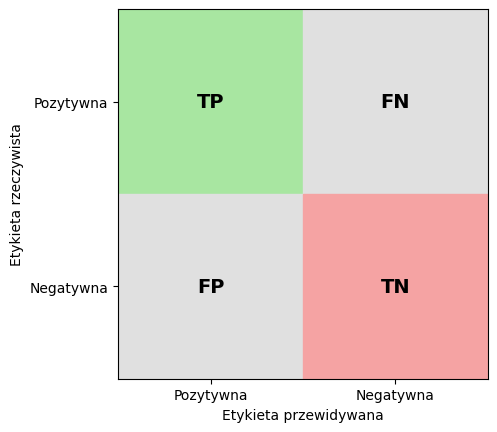
\includegraphics[width=0.5\textwidth]{img/r3/error_matrix.png}
	\caption{Struktura macierzy pomyłek dla klasyfikacji binarnej}
	\label{fig:etykieta-rysunku}
\end{figure}

Wykorzystując wymieniane przypadki, jesteśmy w stanie wyznaczyć metryki jakościowe, które pozwalają na ocenę skuteczności klasyfikatora.

\begin{itemize}
	\item \textbf{Dokładność} - metryka określająca jaki procent przypadków został poprawnie sklasyfikowany. Jest to metryka która jest mocno zalezna od rozkładu klasy. W sytuacji gdy jedna klasas jest znacznie liczniejsza, może ona mocno zakrzywić wyniki. W przypadku klasyfykacji binarnej możemy ją wyznaczyć jako:
	      \begin{equation}
		      \text{Accuracy} = \frac{\text{TP + TN}}{\text{TP + FP + TN + FN}}
	      \end{equation}

	\item \textbf{Precyzja} - miara jakościowa określającą jaki procent przypadków sklasyfikowanych jako osoby z chorobą rzeczywiscie posiadaja arytmię. Prezycja nie zwraca uwagi na przypadki zdrowę, zwraca uwagę jedynie na przypadki z arytmią. Omawianą miarę możemy obliczyć jako:
	      \begin{equation}
		      \text{Precision} = \frac{\text{TP}}{\text{TP + FP}}
	      \end{equation}

	\item \textbf{Czułość} - prawdopodobieństwo ze klasyfikacja będzie poprawna pod warunkiem że dana próbka pochodzi od osoby chorej. Można ją obliczyć ze wzoru:

	      \begin{equation}
		      \text{Recall} = \frac{\text{TP}}{\text{TP + FN}}
	      \end{equation}


	\item \textbf{F-miara} - metryka która łaczy prezycję i czułosć. Wyznacza się jako średnią harmoniczną owych metryk. Ze względu na to, jest ona bardzo wrażliwa na przypadki gdy jedna z metryk jest bardzo niska. Jednak jest ona odporna na nierówny rozkład klas. Wartość F-miary możemy wyznaczyć jako:

	      \begin{equation}
		      \text{F}_1 = \frac{1}{2} \left( \frac{1}{\text{precision}} + \frac{1}{\text{recall}} \right) = \frac{2 \cdot \text{precision} \cdot \text{recall}}{\text{precision} + \text{recall}} = \frac{\text{2TP}}{\text{2TP + FP + FN}}
	      \end{equation}


	\item \textbf{Matthews Correlation Coefficient (MCC)} - miara korelacji binarnej wprowadzona do uczenia maszynowego przez Briana W. Matthewsa~\cite{matthews1975}. Zakres tego współczynnika wynosi od $-1$ do $1$, gdzie $1$ oznacza perfekcyjną klasyfikację, $0$ klasyfikację losową, a $-1$ - całkowicie odwrotną predykcję. MCC jest wskaźnikiem jakościowym odpornym na niezbalansowanie klas i można go obliczyć według wzoru:

	      \begin{equation}
		      \text{MCC} = \frac{\text{TP} \cdot \text{TN} - \text{FP} \cdot \text{FN}}{\sqrt{(\text{TP} + \text{FP})(\text{TP} + \text{FN})(\text{TN} + \text{FP})(\text{TN} + \text{FN})}}
	      \end{equation}
\end{itemize}
\section{Dobór modelu i optymalizacja hiperparametrów}















\chapter{Przetwarzanie i wybrane zbiory danych}
\section{Przegląd wykorzystanych zbiorów danych}
TODO - napisać coś tutaj
\subsection{MIMIC PERform AF Dataset}
Zbiór danych MIMIC PERform AF\cite{mimic_perform_af} został pozyskany z bazy MIMIC-III Waveform Database Matched Subset\cite{mimiciii_waveform_matched}. Zawiera on 20-minutowe zapisy sygnałów fotopletyzmograficznych oraz elektrokardiograficznych, zarejestrowane u 35 ciężko chorych dorosłych pacjentów hospitalizowanych na oddziałach intensywnej terapii. U 19 z tych pacjentów zdiagnozowano migotanie przedsionków, natomiast u pozostałych zapis sygnałów nie wykazywał nieprawidłowości w rytmie serca. Dane zostały zebrane z wykorzystaniem monitora przyłóżkowego, z częstotliwością próbkowania wynoszącą 125 Hz.

\subsection{Zbiór PPG według Liu, Zengding i Zhou et al.}
Dane wykorzystywane w tym zbiorze\cite{liu2022multiclass} zostały zebrane w okresie od marca 2020 do marca 2021 w szpitalu Fuwai w Pekinie, będącym wyspecjalizowaną placówką w zakresie chorób sercowo-naczyniowych. Sygnał fotopletyzmograficzny został początkowo próbkowany z częstotliwością 250 Hz, a następnie poddany procesowi resamplingu do 100 Hz. W celu usunięcia niepożądanych zakłóceń zastosowano filtrację pasmową w zakresie 0.5 - 50 Hz. Przefiltrowany sygnał został następnie podzielony na segmenty 10-sekundowe, przy czym fragmenty zawierające istotne zakłócenia zostały odrzucone.


Cały zbiór danych obejmuje zapisy od 228 pacjentów, co odpowiada łącznie 118 217 segmentom 10-sekundowym. Na potrzeby badań publicznych udostępniono jedynie 46 827 z tych fragmentów. Dane zostały skategoryzowane według pięciu typów arytmii: przedwczesny skurcz komorowy, przedwczesny skurcz przedsionkowy, tachykardia komorowa, tachykardia nadkomorowa oraz migotanie przedsionków.

\subsection{PhysioNet/CinC Challenge 2015}
test\cite{physionet_challenge_2015} Jest zbiorem użytym w konkursie majacym na celu stworzenie algorytmu redukującego ilość fałszych alarmów podczas detekcji arytmii serca. Dane pochodzą z czterech losowo wybranch, szpitali w Stanach Zjednoczonych oraz Europie. Udostępniona część zbioru zawiera 750 nagrań. Sygnały zostały próbkowane z częstotliwością 250Hz oraz przefiltrowane filtrem pasmowym 0.05 - 40Hz
\subsection{Dane syntetyczne}
W celu wzbogacenia zbiorów danych, zdecydowano użyć się danych syntetycznych wygenerowanych przy użyciu generatora sygnałów PPG i ECG z epizodami arrytmi\cite{solosenko2022}. Zastosowany symulator umożliwia pełną kontrolę nad procesem generowania sygnałów. Użytkownik ma możliwość definiowania szeregu parametrów determinujących charakterystykę sygnału, w tym: rodzaj arrytmi, mediane dłguości epizodów arytmi, obciążenie arytmią które determinuje łączny czas kiedy występuje arytmia, wskaźnik przedwczesnychskurczów przedsionkowych czy rodzaj pulsu zdefiniowany przez Dawber et al\cite{dawber1973dicrotic}.
\begin{figure}[!h]
	\centering
	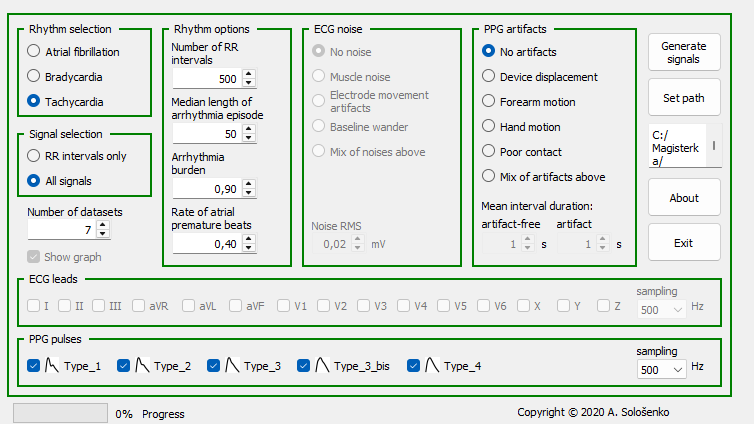
\includegraphics[width=1\textwidth]{img/r4/symulator_GUI.png}
	\caption{GUI użytego symulatora}
	\label{fig:etykieta-rysunku}
\end{figure}\\

W ramach eksperymentu wygenerowano pięć syntetycznych podzbiorów danych, z których każdy został zasymulowany z częstotliwością próbkowania równą 500 Hz oraz zawierał sygnały odpowiadające 500 kolejnym interwałom RR. Każdy ze zbiorów zawierał równą ilośc przypadków bradycardii, tachycardii i migotania przedsionków. Zawierał się w nich także każdy rodzaj pulsu PPG. Zdecydowano się nie wykorzystywać możliwości generowania sygnałów z szumem.

Poszczególne podzbiory różniły się parametrami charakterystycznymi dla przebiegu arytmii:

\begin{table}[ht]
	\centering
	\caption{Porównanie parametrów podzbiorów danych syntetycznych}
	\begin{tabular}{
			@{}c
			S[table-format=2.0]
			S[table-format=1.1]
			S[table-format=1.2]
			@{}
		}
		\toprule
		Zbiór &
		\multicolumn{1}{c}{\makecell{Mediana długości        \\ epizodu arytmii}} &
		\multicolumn{1}{c}{\makecell{Obciążenie              \\ arytmią}} &
		\multicolumn{1}{c}{\makecell{Wskaźnik przedwczesnych \\ skurczów przedsionkowych}} \\
		\midrule
		1     & 3  & 0.1 & 0.05                              \\
		2     & 10 & 0.3 & 0.10                              \\
		3     & 5  & 0.5 & 0.10                              \\
		4     & 30 & 0.4 & 0.20                              \\
		5     & 50 & 0.9 & 0.40                              \\
		\bottomrule
	\end{tabular}
\end{table}

Każdy ze zbiorów ma symulować inny rodzaj arytmi:
\begin{itemize}
	\item Zbiór 1 - Rzadkie występowanie krótkich epizodów arytmi
	\item Zbiór 2 - Umiarkowane występowanie z umiarkowaną liczbą przedwczesnych skórczy
	\item Zbiór 3 - Wysokie występowanie arytmi z krótkimi epizodami
	\item Zbiór 4 - Długie, częste epizody arytmi.
	\item Zbiór 5 - Niemal ciągła arytmia
\end{itemize}

Dzięki zastosowanemu symulatorowi, wygenerowane dane syntetyczne mogą stanowić cenne źródło informacji dla przyszłych modeli klasyfikacyjnych. Umożliwiają one nie tylko lepsze zrozumienie przypadków odstających, ale również wspierają proces uczenia modeli w scenariuszach bardziej typowych, odpowiadających klasycznym przypadkom klinicznym.

\section{Przetwarzanie wstępne}
Pomimo wysokiej jakości wybranych zbiorów danych, ich bezpośrednie wykorzystanie w procesie klasyfikacji wymaga zastosowania wieloetapowego przetwarzania wstępnego. Głównym celem tych transformacji jest ujednolicenie charakterystyki sygnałów pochodzących z różnych źródeł oraz przygotowanie reprezentatywnego wektora cech, który może zostać wykorzystany w procesie uczenia klasyfikatorów.\\

\newpage
Pierwszym etapem przetwarzania wstępnego sygnału jest jego filtracja. W tym celu zastosowano filtr pasmowo-przepustowy o częstotliwościach granicznych 0.5 Hz oraz 40 Hz. Głównym celem tak dobranego filtra jest eliminacja zakłóceń pochodzących spoza pasma istotnego z punktu widzenia analizy sygnałów PPG. Dolne ograniczenie pozwala zmniejszyć wpływ ruchu pacjenta czy zmiane położenia czujnika, natomiast górna granica redukuje wpływ wysokoczęstotliwościowych zakłóceń, takich jak zakłócenia elektromagnetyczne.\\

Drugim istotnym etapem przetwarzania wstępnego była zmiana częstotliwości próbkowania sygnałów. Zdecydowano się na jednolitą częstotliwość 100 Hz, co odpowiada najniższej wartości występującej wśród wykorzystanych zbiorów danych. Ujednolicenie próbkowania do tej wartości niesie ze sobą kilka korzyści. Po pierwsze, redukcja liczby próbek skutkuje zmniejszeniem rozmiaru danych, co przekłada się na krótszy czas ich przetwarzania jak i nauki modeli w sposób bezcechowych.\\

Kolejnym krokiem w procesie przetwarzania wstępnego była normalizacja sygnału do przedziału $[0, 1]$. Wykorzystane zbiory danych charakteryzowały się zróżnicowanym zakresem wartości amplitud, co mogłoby negatywnie wpłynąć zarówno na proces uczenia cechowego, jak i bezcechowego. Niejednorodna skala danych może prowadzić do dominacji niektórych sygnałów lub cech w trakcie uczenia. W celu minimalizacji tego efektu, zdecydowano się na niezależną normalizację każdego sygnału osobno.\\

Z uwagi na fakt, że zbiór danych opracowany przez Liu, Zengding i Zhou et al.\cite{liu2022multiclass} składa się z 10-sekundowych segmentów sygnału, zdecydowano o ujednoliceniu długości wszystkich pozostałych próbek poprzez ich podział na fragmenty o identycznym czasie trwania. Segmentacja została przeprowadzona po wcześniejszym przeskalowaniu częstotliwości próbkowania do 100 Hz, co oznacza, że każdy 10-sekundowy segment zawiera dokładnie 1000 próbek. Próbki te, zostaną wykorzytane do bezcechowej nauki klasyfikatorów.\\

Ostatnim etapem przetwarznia wstępnego jest wybranie oraz ekstrakcja cech. Proces ten zostanie omówiony dokładnie w rozdziale \ref{Ekstrakcja cech}

\begin{figure}[!h]
	\caption{Schemat przetwarznia wstępnego}

	\begin{tikzpicture}
		% Bloki
		\node[draw, align=center, minimum width=2cm, minimum height=1.1cm] (B) at (0.5,0) {Filtr\\pasmowy};
		\node[draw, align=center, minimum width=2cm, minimum height=1.1cm] (C) at (3.05,0) {Resampler};
		\node[draw, align=center, minimum width=2cm, minimum height=1.1cm] (D) at (5.9,0) {Normalizator};
		\node[draw, align=center, minimum width=2cm, minimum height=1.1cm] (E) at (8.9,0) {Segmentator};
		\node[draw, align=center, minimum width=2cm, minimum height=1.1cm] (F) at (11.7,0) {Ekstraktor\\cech};

		% Strzałki
		\draw[->] (-2,0) -- (B.west)
		node[midway, above, align=center] {Bazowy\\sygnał};
		\draw[->] (B) -- (C) node[midway] {};
		\draw[->] (C) -- (D) node[midway] {};
		\draw[->] (D) -- (E) node[midway] {};
		\draw[->] (E) -- (F.west) node[midway] {};
		\draw[->] (F.east) -- (14,0)
		node[midway, above, align=center]{Wektor\\cech};
		\draw[-] (E.east) -- (11,-2.5)
		node[midway, above, align=center]{};
		\draw[->] (11,-2.5) -- (14,-2.5)
		node[midway, above, align=center]{Segmentowany\\sygnał};

	\end{tikzpicture}
\end{figure}

\newpage
\section{Ekstrakcja cech}
\label{Ekstrakcja cech}
Zdecydowano się na wybór czterech głównych domen analizy, z których każda interpretuje sygnał PPG z innej perspektywy, umożliwiając wydobycie zróżnicowanych informacji. Niezależnie od wybranej domeny, we wszystkich przypadkach zastosowano zestaw podstawowych miar statystycznych, które zostały wyekstrahowane z przekształconych sygnałów:
\begin{itemize}
	\item Średnia arytmetyczna,
	\item Mediana,
	\item Odchylenie standardowe,
	\item Wariancja,
	\item Rozstęp międzykwartylowy,
\end{itemize}

\subsection{Cechy z domeny czasu}
Pierwszą z wybranych domen, interpretuje sygnał jako funkcję ciągłą w czasie. Domena czasu trakuje kolejne próbki czasowe jako kolejne wartości funkcji aplitudy. Domena ta bezpośrednio analizuje sygnału w jej pierwotnej postaci, gdzie $x = \{x_1, x_2, \ldots, x_n\}$. W tej przestrzeni, zdecydowano się na wybranie następujących cech:
\begin{itemize}
	\item \textbf{Skośność} - miara asymetrii sygnału:
	      \begin{equation}
		      \frac{1}{N} \sum_{i=1}^{N} \left( \frac{x_i - \bar{x}}{\sigma} \right)^3
	      \end{equation}
	      gdzie:
	      \begin{itemize}
		      \item \( \bar{x} \) - średnia arytmetyczna.
		      \item \( \sigma \) - odchylenie standardowe sygnału.
	      \end{itemize}
	\item \textbf{Współczynnik zmienności} -  względna miara zróżnicowania sygnału:
	      \begin{equation}
		      \text{CV} = \frac{\sigma}{\bar{x}}
	      \end{equation}
	\item \textbf{Średnie odchylenie bezwzględne} - bezwzgledna miara zróżnicowania sygnału:
	      \begin{equation}
		      \text{MAD} = \frac{1}{n} \sum_{i=1}^{n} \left| x_i - \bar{x} \right|
	      \end{equation}

	\item \textbf{Entropia Shannona} - miara niepewności sygnału:
	      \begin{equation}
		      H = -\sum_{i=1}^{N} p_i \mathrm{log}_{2} p_i
	      \end{equation}
	      gdzie:
	      \begin{itemize}
		      \item \( p_i \) - prawdopodobieństwo wystąpienia \( i \)-tej wartości sygnału.
	      \end{itemize}





\end{itemize}


\subsection{Cechy różnicowe}
Kolejną z wybranych domen jest domena cech różnicowych, w której sygnał nie jest bezpośrednio intereptowany jako kolejne wartości amplitudy, tylko poprzez różnice zmian między kolejnymi próbkami $\Delta x = \{x_2 - x_1,\, x_3 - x_2,\, \ldots,\, x_n - x_{n-1}\}$. Cechy wyekstrachowane z tej domeny:
\begin{itemize}
	\setcounter{enumi}{4}
	\item \textbf{Procent dodatnich różnic} - odsetek dodatkich róznic kolejnych wartości sygnału

	      \begin{equation}
		      \frac{100}{N-1} \sum_{i=1}^{N-1} \delta(\Delta x > 0)
	      \end{equation}
	      gdzie:
	      \begin{itemize}
		      \item \( \delta(\cdot) \) - funkcja wskaźnikowa, równa 1 gdy warunek jest spełniony, 0 w przeciwnym wypadku.
	      \end{itemize}
	\item \textbf{Średnia wartość bezwzględna różnic:}
	      \begin{equation}
		      \frac{1}{N-1} \sum_{i=1}^{N-1} |\Delta x|
	      \end{equation}

	\item \textbf{Pierwiastek średniokwadratowy różnic} - miara zmienności rytmu serca, która odzwierciedla aktywność układu przywspółczulnego:\cite{Farokhipour2023}
	      \begin{equation}
		      \text{RMSSD} = \sqrt{ \frac{1}{N-1} \sum_{i=1}^{N-1} (\Delta x)^2 }
	      \end{equation}

	\item \textbf{Znormalizowane średnie odchylenie bezwzględne różnic} - ocenia lokalną dynamikę zmian sygnału:
	      \begin{equation}
		      \frac{1}{N-1} \sum_{i=1}^{N-1} \frac{|\Delta x|}{\bar{x}}
	      \end{equation}

	\item \textbf{Znormalizowana suma bezwzględnych różnic:}

	      \begin{equation}
		      \frac{\sum_{i=1}^{N-1} |\Delta x|}{\sum_{i=1}^{N} |x_i|}
	      \end{equation}

\end{itemize}


\subsection{Cechy częstotliwościowe}
Ostatnią wybraną domeną jest domena częstotliwościowa. W tej domenie, sygnał jest przekszłcany przy użyciu transoframty Fouriera, aby uzyskać jego rozkład mocny w zależności częstotliwości $P_{xx}(f)$, gdzie $f$ oznacza częstotliwość. Analiza cech częstotliwościowych, pozwala identyfikować składowe dominujące jak i nieregularności. W tej domenie zdecydowano się na ekstrakcję następujących cech:
\begin{itemize}
	\setcounter{enumi}{9}
	\item \textbf{Maksymalny szczyt widmowy}
	      \begin{equation}
		      f_{\max} = f \bigl( \arg\max_{f} P_{xx}(f) \bigr)
	      \end{equation}


	\item \textbf{Kurtoza widma} - spłaszczenie sygnału:
	      \begin{equation}
		      \text{kurt}(P_{xx}) = \frac{1}{M} \sum_{j=1}^M \left( \frac{P_{xx}(f_j) - \overline{P_{xx}}}{\sigma_{P_{xx}}} \right)^4
	      \end{equation}

	\item \textbf{Udział wysokich szczytów widma}
	      \begin{equation}
		      \frac{\sum_{J=1}^{M} \delta(P_{xx}(f_j) > \overline{P_{xx}} )}{M}
	      \end{equation}
\end{itemize}



\chapter{Detekcja arytmii serca}
\section{Architektura i konfiguracja modeli}
\section{Walidacja wyników}
\subsection{Walidacja holdout}
\subsection{Walidacja K-Fold}
\section{Analiza wyników}

\chapter{Podsumowanie i wnioski}


% W całym dokumencie powinny znajdować się odniesienia do zawartych w nim ilustracji (rys. \ref{fig:2}).

% \begin{figure}
% 	\centering
% 	\begin{tikzpicture}
% 		\begin{axis}[
% 				y tick label style={
% 						/pgf/number format/.cd,
% 						fixed,   % po zakomentowaniu os rzednych jest indeksowana wykladniczo
% 						fixed zerofill, % 1.0 zamiast 1
% 						precision=1,
% 						/tikz/.cd
% 					},
% 				x tick label style={
% 						/pgf/number format/.cd,
% 						fixed,
% 						fixed zerofill,
% 						precision=2,
% 						/tikz/.cd
% 					}
% 			]
% 			\addplot [domain=0.0:0.1] {rnd};
% 		\end{axis}
% 	\end{tikzpicture}
% 	\caption{Wykres przebiegu funkcji.} % Podpis jest zawsze POD rysunkiem.
% 	\label{fig:2}
% \end{figure}


%%%%%%%%%%%%%%%%%%%%%
%% RYSUNEK Z PLIKU
%
%\begin{figure}
%\centering
%
\includegraphics[width=0.5\textwidth]{./politechnika_sl_logo_bw_pion_pl.pdf}
%\caption{Podpis rysunku zawsze pod rysunkiem.}
%\label{fig:etykieta-rysunku}
%\end{figure}
%Rys. \ref{fig:etykieta-rysunku} przestawia …
%%%%%%%%%%%%%%%%%%%%%
%
%%%%%%%%%%%%%%%%%%%%%
%% WIELE RYSUNKÓW 
%
%\begin{figure}
%\centering
%\begin{subfigure}{0.4\textwidth}
%    
\includegraphics[width=\textwidth]{./politechnika_sl_logo_bw_pion_pl.pdf}
%    \caption{Lewy górny rysunek.}
%    \label{fig:lewy-gorny}
%\end{subfigure}
%\hfill
%\begin{subfigure}{0.4\textwidth}
%    
\includegraphics[width=\textwidth]{./politechnika_sl_logo_bw_pion_pl.pdf}
%    \caption{Prawy górny rysunek.}
%    \label{fig:prawy-gorny}
%\end{subfigure}
%
%\begin{subfigure}{0.4\textwidth}
%    
\includegraphics[width=\textwidth]{./politechnika_sl_logo_bw_pion_pl.pdf}
%    \caption{Lewy dolny rysunek.}
%    \label{fig:lewy-dolny}
%\end{subfigure}
%\hfill
%\begin{subfigure}{0.4\textwidth}
%    
\includegraphics[width=\textwidth]{./politechnika_sl_logo_bw_pion_pl.pdf}
%    \caption{Prawy dolny rysunek.}
%    \label{fig:prawy-dolny}
%\end{subfigure}
%        
%\caption{Wspólny podpis kilku rysunków.}
%\label{fig:wiele-rysunkow}
%\end{figure}
%Rys. \ref{fig:wiele-rysunkow} przestawia wiele ważnych informacji, np. rys. \ref{fig:prawy-gorny} jest na prawo u góry.
%%%%%%%%%%%%%%%%%%%%%


% Tekst dokumentu powinien również zawierać odniesienia do tabel (tab. \ref{id:tab:wyniki}).

% \begin{table}
% 	\centering
% 	\caption{Opis tabeli nad nią.}
% 	\label{id:tab:wyniki}
% 	\begin{tabular}{rrrrrrrr}
% 		\toprule
% 		        & \multicolumn{7}{c}{metoda}                                                                                                                                  \\
% 		\cmidrule{2-8}
% 		        &                            &         & \multicolumn{3}{c}{alg. 3} & \multicolumn{2}{c}{alg. 4, $\gamma = 2$}                                                \\
% 		\cmidrule(r){4-6}\cmidrule(r){7-8}
% 		$\zeta$ & alg. 1                     & alg. 2  & $\alpha= 1.5$              & $\alpha= 2$                              & $\alpha= 3$ & $\beta = 0.1$ & $\beta = -0.1$ \\
% 		\midrule
% 		0       & 8.3250                     & 1.45305 & 7.5791                     & 14.8517                                  & 20.0028     & 1.16396       & 1.1365         \\
% 		5       & 0.6111                     & 2.27126 & 6.9952                     & 13.8560                                  & 18.6064     & 1.18659       & 1.1630         \\
% 		10      & 11.6126                    & 2.69218 & 6.2520                     & 12.5202                                  & 16.8278     & 1.23180       & 1.2045         \\
% 		15      & 0.5665                     & 2.95046 & 5.7753                     & 11.4588                                  & 15.4837     & 1.25131       & 1.2614         \\
% 		20      & 15.8728                    & 3.07225 & 5.3071                     & 10.3935                                  & 13.8738     & 1.25307       & 1.2217         \\
% 		25      & 0.9791                     & 3.19034 & 5.4575                     & 9.9533                                   & 13.0721     & 1.27104       & 1.2640         \\
% 		30      & 2.0228                     & 3.27474 & 5.7461                     & 9.7164                                   & 12.2637     & 1.33404       & 1.3209         \\
% 		35      & 13.4210                    & 3.36086 & 6.6735                     & 10.0442                                  & 12.0270     & 1.35385       & 1.3059         \\
% 		40      & 13.2226                    & 3.36420 & 7.7248                     & 10.4495                                  & 12.0379     & 1.34919       & 1.2768         \\
% 		45      & 12.8445                    & 3.47436 & 8.5539                     & 10.8552                                  & 12.2773     & 1.42303       & 1.4362         \\
% 		50      & 12.9245                    & 3.58228 & 9.2702                     & 11.2183                                  & 12.3990     & 1.40922       & 1.3724         \\
% 		\bottomrule
% 	\end{tabular}
% \end{table}


%\chapter{[Przedmiot pracy]}
%
%\begin{itemize}
%\item  Jak ja rozwiązuję problem?
%\begin{itemize}
%\item rozwiązanie zaproponowane przez dyplomanta
%\item analiza teoretyczna rozwiązania
%\item uzasadnienie wyboru zastosowanych metod, algorytmów, narzędzi
%\end{itemize}
%\end{itemize}


% TODO
%
% 
%
%Rozdział przedstawia przeprowadzone badania. Jest to zasadnicza część i~musi wyraźnie dominować w~pracy.
%Badania i analizę wyników należy przeprowadzić, tak jak jest przyjęte w środowisku naukowym (na przykład korzystanie z danych benchmarkowych, walidacja krzyżowa, zapewnienie powtarzalności testów itd). 
%
%\section{Metodyka badań}
%
%\begin{itemize}
%\item opis metodyki badań
%\item opis stanowiska badawczego (opis interfejsu aplikacji badawczych -- w~załączniku)
%\end{itemize}
%
%
%\section{Zbiory danych}
%
%\begin{itemize}
%\item opis danych
%\end{itemize}
%
%
%\section{Wyniki}
%
%\begin{itemize}
%\item prezentacja wyników, opracowanie i poszerzona dyskusja  wyników, wnioski
%\end{itemize}
%
% 
%\begin{table}
%\centering
%\caption{Opis tabeli nad nią.}
%\label{id:tab:wyniki}
%\begin{tabular}{rrrrrrrr}
%\toprule
%	         &                                     \multicolumn{7}{c}{metoda}                                      \\
%	         \cmidrule{2-8}
%	         &         &         &        \multicolumn{3}{c}{alg. 3}        & \multicolumn{2}{c}{alg. 4, $\gamma = 2$} \\
%	         \cmidrule(r){4-6}\cmidrule(r){7-8}
%	$\zeta$ &     alg. 1 &   alg. 2 & $\alpha= 1.5$ & $\alpha= 2$ & $\alpha= 3$ &   $\beta = 0.1$  &   $\beta = -0.1$ \\
%\midrule
%	       0 &  8.3250 & 1.45305 &       7.5791 &    14.8517 &    20.0028 & 1.16396 &                       1.1365 \\
%	       5 &  0.6111 & 2.27126 &       6.9952 &    13.8560 &    18.6064 & 1.18659 &                       1.1630 \\
%	      10 & 11.6126 & 2.69218 &       6.2520 &    12.5202 &    16.8278 & 1.23180 &                       1.2045 \\
%	      15 &  0.5665 & 2.95046 &       5.7753 &    11.4588 &    15.4837 & 1.25131 &                       1.2614 \\
%	      20 & 15.8728 & 3.07225 &       5.3071 &    10.3935 &    13.8738 & 1.25307 &                       1.2217 \\
%	      25 &  0.9791 & 3.19034 &       5.4575 &     9.9533 &    13.0721 & 1.27104 &                       1.2640 \\
%	      30 &  2.0228 & 3.27474 &       5.7461 &     9.7164 &    12.2637 & 1.33404 &                       1.3209 \\
%	      35 & 13.4210 & 3.36086 &       6.6735 &    10.0442 &    12.0270 & 1.35385 &                       1.3059 \\
%	      40 & 13.2226 & 3.36420 &       7.7248 &    10.4495 &    12.0379 & 1.34919 &                       1.2768 \\
%	      45 & 12.8445 & 3.47436 &       8.5539 &    10.8552 &    12.2773 & 1.42303 &                       1.4362 \\
%	      50 & 12.9245 & 3.58228 &       9.2702 &    11.2183 &    12.3990 & 1.40922 &                       1.3724 \\
%\bottomrule
%\end{tabular}
%\end{table}  
%
%
% 
%\begin{figure}
%\centering
%\begin{tikzpicture}
%\begin{axis}[
%    y tick label style={
%        /pgf/number format/.cd,
%            fixed,   % po zakomentowaniu os rzednych jest indeksowana wykladniczo
%            fixed zerofill, % 1.0 zamiast 1
%            precision=1,
%        /tikz/.cd
%    },
%    x tick label style={
%        /pgf/number format/.cd,
%            fixed,
%            fixed zerofill,
%            precision=2,
%        /tikz/.cd
%    }
%]
%\addplot [domain=0.0:0.1] {rnd};
%\end{axis} 
%\end{tikzpicture}
%\caption{Podpis rysunku po rysunkiem.}
%\label{fig:2}
%\end{figure}
%
%
%\begin{figure}
%\begin{lstlisting}
%if (_nClusters < 1)
%	throw std::string ("unknown number of clusters");
%if (_nIterations < 1 and _epsilon < 0)
%	throw std::string ("You should set a maximal number of iteration or minimal difference -- epsilon.");
%if (_nIterations > 0 and _epsilon > 0)
%	throw std::string ("Both number of iterations and minimal epsilon set -- you should set either number of iterations or minimal epsilon.");
%\end{lstlisting}
%\caption{Przykład pseudokodu}
%\end{figure}


% TODO



%\begin{itemize}
%\item Jaki problem rozwiązałæm?
%\item Jak ten problem rozwiązałæm?
%\item Jakie są dobre i słabe strony mojego rozwiązania?
%\item Czy mogę sformułować jakieś rekomendacje?
%\end{itemize}

\begin{itemize}
	\item syntetyczny opis wykonanych prac
	\item wnioski
	\item możliwość rozwoju, kontynuacji prac, potencjalne nowe kierunki
	\item Czy cel pracy zrealizowany?
\end{itemize}



\backmatter

%\bibliographystyle{plplain}  % bibtex
%\bibliography{biblio} % bibtex
\printbibliography           % biblatex
\addcontentsline{toc}{chapter}{Bibliografia}

\begin{appendices}

	% TODO


	% TODO
	\chapter{Spis skrótów i symboli}

	\begin{itemize}
		\item[PPG] Sygnał fotopletyzmograficzny
		\item[$\bar{x}$] Średnia wartość sygnału
		\item[$\sigma$] Odchylenie standardowe
		\item[H] Entropie Shannona
		\item[E] Energia
		\item[RMSSD] Pierwiastek średniokwadratowy różnic
		\item[kurt] Kurtoza widma
		\item[MVC] model -- widok -- kontroler (ang. \english{model--view--controller})
		\item[$\mu$] stopnień przyleżności do zbioru
		\item[$\mathbb{E}$] zbiór krawędzi grafu
		\item[$\mathcal{L}$] transformata Laplace'a
	\end{itemize}

	% TODO
	\chapter{Lista dodatkowych plików, uzupełniających tekst pracy}

	W systemie do pracy dołączono dodatkowe pliki zawierające:
	\begin{itemize}
		\item źródła programu,
		\item zbiory danych użyte w~eksperymentach,
		\item film pokazujący działanie opracowanego oprogramowania lub zaprojektowanego i wykonanego urządzenia,
		\item itp.
	\end{itemize}


	\listoffigures
	\addcontentsline{toc}{chapter}{Spis rysunków}
	\listoftables
	\addcontentsline{toc}{chapter}{Spis tabel}

\end{appendices}

\end{document}


%% Finis coronat opus.

